\documentclass{article}
\usepackage[utf8]{inputenc}
\usepackage[german]{babel}
\usepackage{graphicx} 
\usepackage{amsmath, amssymb}
\usepackage[section]{placeins}
\usepackage[square,numbers]{natbib}
\bibliographystyle{abbrvnat}
\usepackage{mathtools}
\usepackage{caption}
\usepackage{subcaption}
\usepackage{cleveref}

\title{Aufbau und Justage eines Leckstrahlmikroskopes zum Nachweis des plasmonischen Spin-Hall-Effektes}
\author{Hanno Christiansen}
\date{März 2021}

\begin{document}
	
\maketitle
\tableofcontents

\section{Einführung}
\section{Theorie}
	\subsection{Oberflächen-Plasmon-Polariton (SPP)}		
	Ein Oberflächen-Plasmon-Polariton (engl. Surface-Plasmon-Polariton SPP) ist das quantisierte Quasiteilchen, der an das elektromagnetischen Feld gekoppelten Elektronen-Dichte-Oszillation, an einer Dielektrikums-Metall-Grenzschicht. Durch die spezielle Form dieser Geometrie ist es möglich, trotz des rein longitudinalen Charakters der Elektronen-Dichte-Oszillation, ein elektromagnetisches Feld mit transversalen Komponenten zu erzeugen. Diese transversalen Komponenten sind notwendig, um  damit eine Kopplung an das rein transversale elektromagnetische Feld des Vakuums tendenziell zu ermöglichen. Die einfachste Geometrie in der SPPs auftreten können ist ein Zwei-Schichtsystem. Der Halbraum oberhalb der $xy$-Ebene mit $z>0$ sei von einem Dielektrikum mit der Dielektrizitätskonstante $\epsilon_D$ ausgefüllt. Der Halbraum unterhalb der $xy$-Ebene mit $z<0$ sei von einem Metall mit der im allgemeinen komplexen Dielektrischen-Funktion $\epsilon(\omega)$ ausgefüllt. An der Grenzschicht zwischen diesen beiden Halbräumen können SPPs propagieren. Um nun einige Charakteristische Eigenschaften von SPPs zu erläutern, gehe ich davon aus, dass das SPP entlang der $x$-Achse propagiert und entlang der y-Achse homogen ist. So wird das Problem effektiv 2-dimensional. Wie in \cite{Maier.2007} gezeigt, lassen sich die elektromagnetischen Felder eines SPPs in dieser einfachen Geometrie durch folgende Ausdrücke beschreiben:
	\begin{equation}
		\label{eq:electric_field_spp}
		\vec{E}_n = \begin{pmatrix} 1 \\ 0 \\ \pm k_{\mathrm{spp}}/k_{z,n} \end{pmatrix} E_0 \exp\left(i(k_{\mathrm{spp}}x + k_{z, n}|z|-\omega t)\right)	
	\end{equation}
	\begin{equation}
		\label{eq:magnetic_field_spp}
		\vec{H}_n = \begin{pmatrix} 0 \\ 1 \\ 0 \end{pmatrix} H_0 \exp\left(i(k_{\mathrm{spp}}x + k_{z, n}|z|-\omega t)\right)
	\end{equation}
	Der Index $n$ beschreibt hierbei das Material($M$ für das Metall, $D$ für das Dielektrikum). Das $\pm$ ist $+$ für das Metall und  $-$ für das Dielektrikum. $\omega$ ist die Winkelfrequenz der Anregung. $k_{\mathrm{spp}}$ ist der im allgemeinen komplexe Wellenvektor der Anregung.  $k_{\mathrm{spp}}$ ist für beide Medien gleich. Der Realteil $\operatorname{\mathbb{R}e}\{k_{\mathrm{spp}}\}$ des komplexen Wellenvektors lässt sich in die Wellenlänge $\lambda_{\mathrm{spp}} = 2\pi/ \operatorname{\mathbb{R}e}\{k_{\mathrm{spp}}\} $ des SPP umrechnen. Der Imaginärteil $\operatorname{\mathbb{I}m}\{k_{\mathrm{spp}}\}$ beschreibt das Dämpfungsverhalten des SPP entlang der Ausbreitungsrichtung. Es lässt sich über $\L_{\mathrm{spp}} = 1/(2\operatorname{\mathbb{I}m}\{k_{\mathrm{spp}}\})$ eine Propagationslänge definieren. Nachdem das SPP eine Propagationslänge zurückgelegt hat, sind die ursprünglichen Intensitäten des SPP auf $1/\mathrm{e}$ ihres ursprünglichen Betrages zurückgegangen.
	
	Analog beschreibt $\operatorname{\mathbb{R}e}\{k_{z, n}\}$ den Exponentiellen-Abfall der Anregung, wenn man sich von der Grenzfläche entfernt. Hier lassen sich die Eindringtiefen $\delta_{M,D}$ definieren, die angeben nach welcher Entfernung in z-Richtung die ursprungliche Feldstärke auf $1/\mathrm{e}$ abgeklungen ist. Das SPP hat sowohl transversale, als auch longitudinale Komponenten des Elektrischen Feldes. Das magnetische Feld ist rein transversal. Daher spricht man auch von einer Transversal-Magnetischen Anregung (TM).
	Der quantitativer Verlauf des elektrischen Feldes für ein rein reelles $k_{\mathrm{spp}}$ und ein rein imaginäres $k_{z, n}$ ist in Abb. \ref{fig:electric_field_spp} dargestellt.
	\begin{figure}[htbp] 
		\centering
		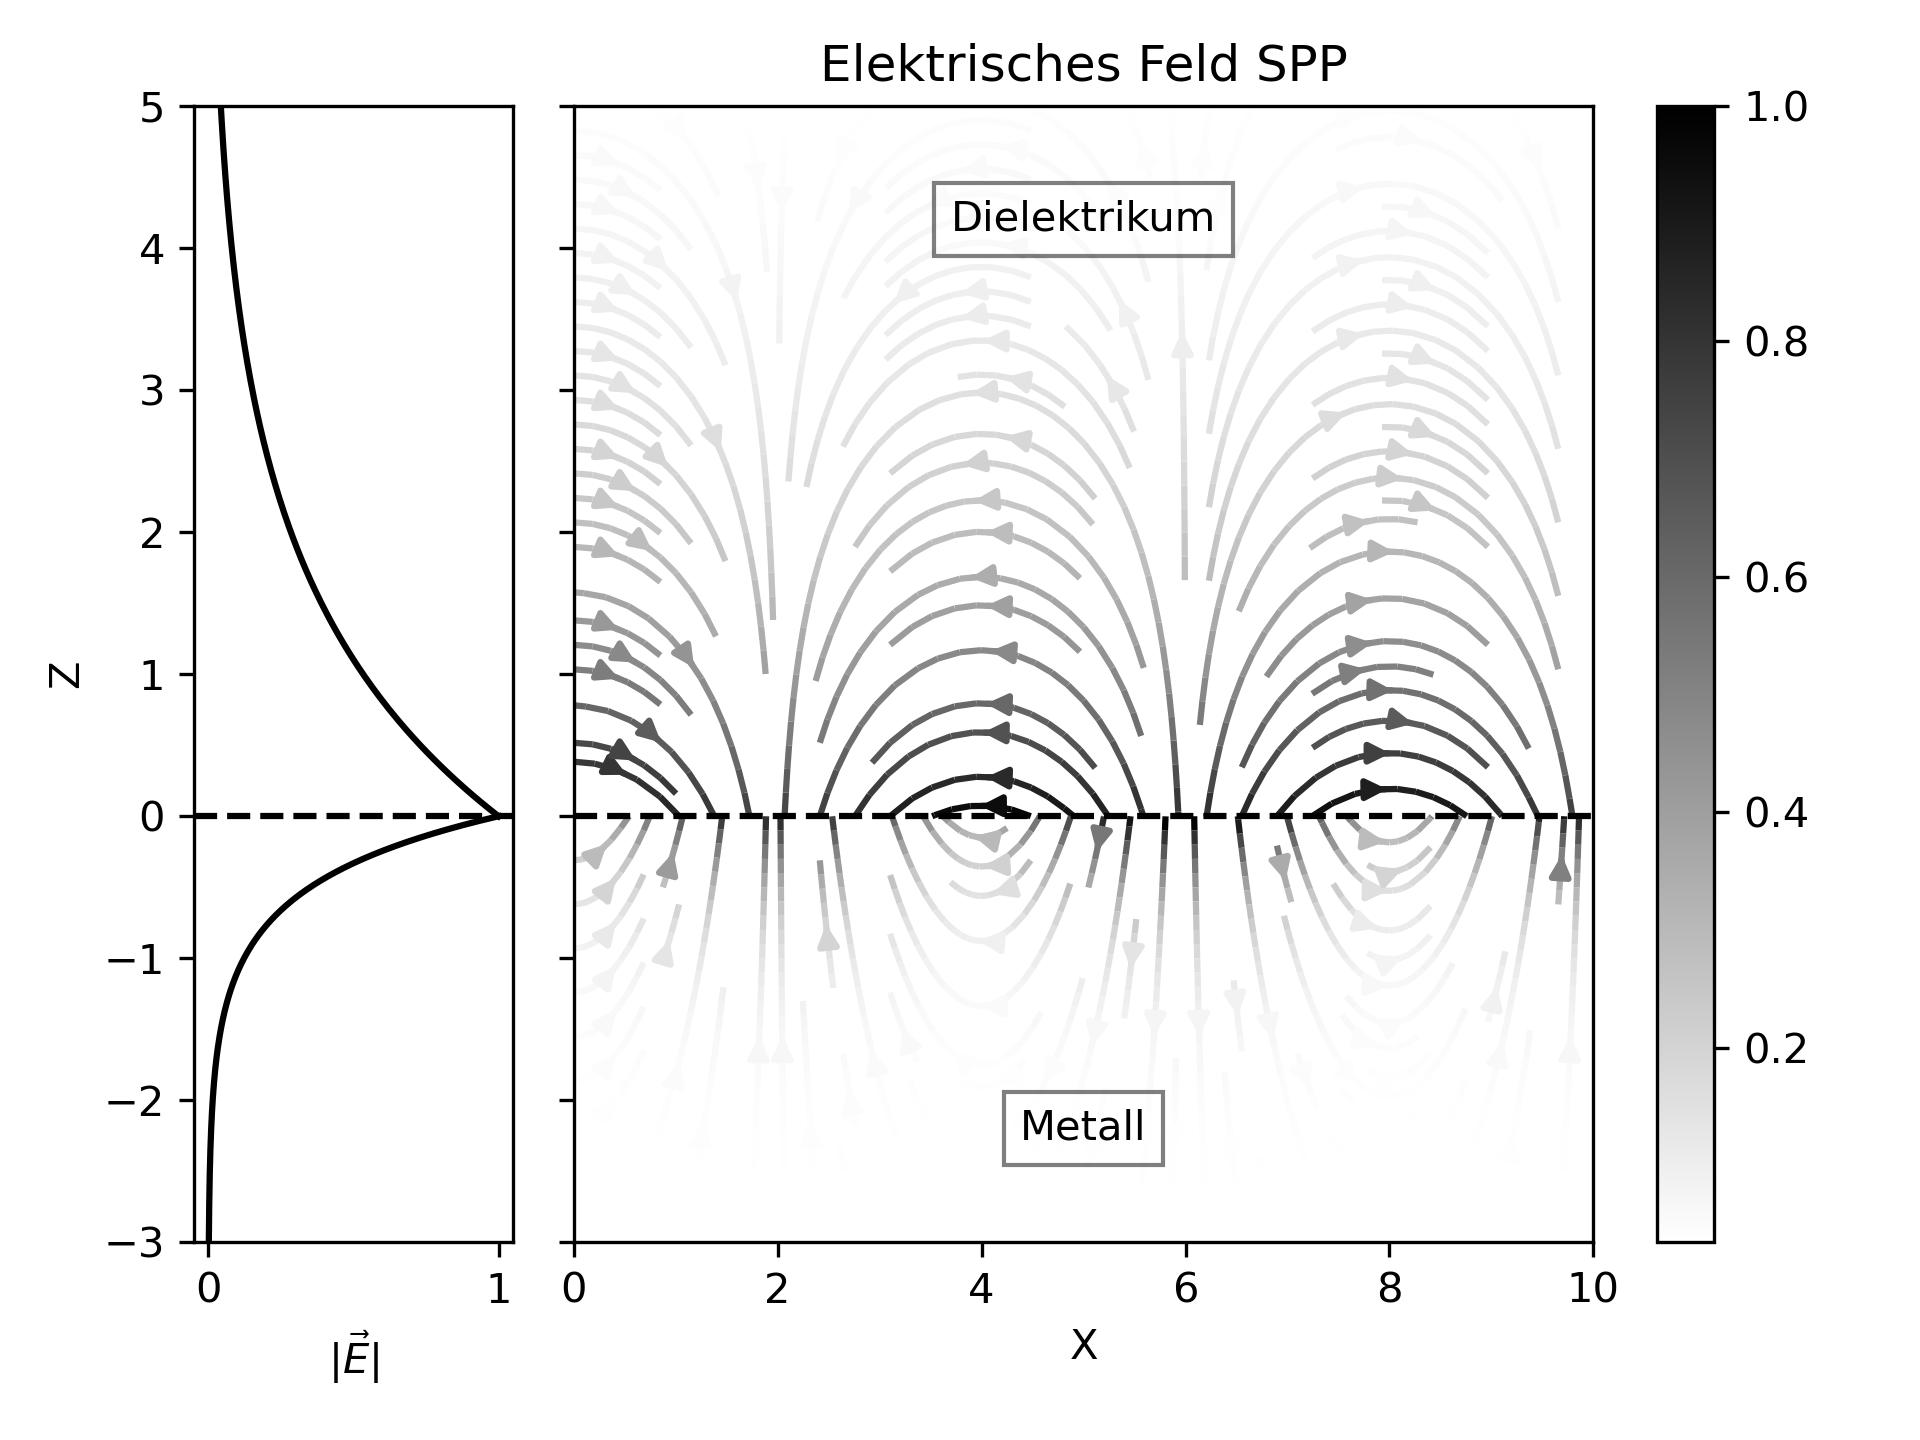
\includegraphics[width=1\textwidth]{figures/E_Feld_SPP.png}
		\caption{Quantitativer Verlauf des Elektrischen Feldes eines SPPs entlang einer Metall-Dielektrikums-Grenzschicht in der  xy-Ebene mit Ausbreitungsrichtung in positiver x-Richtung}
		\label{fig:electric_field_spp}
	\end{figure}

	\subsubsection{Dispersion}
	Die Herleitung der Dispersionsrelation orientiert sich an den Ausführungen in \cite[pp.~261--ff]{Fox.2020} und kann dort im Detail nachvollzogen werden. Ich beschränke mich hier auf eine kurze Beschreibung des Vorgehens.
	Damit die oben angesetzten elektromagnetischen Felder \eqref{eq:electric_field_spp}, \eqref{eq:magnetic_field_spp}  die Maxwellgleichungen \eqref{eq:maxwell} und die Randbedingungen an der Grenzschicht erfüllen, müssen die Bedingungen \eqref{eq:condition_spp_1},  \eqref{eq:condition_spp_2} gelten. (Hierbei handelt es sich um den Spezialfall nicht magnetischer Materialien.)
	\begin{align}
		\label{eq:maxwell}	
		&\vec{\nabla}\cdot\vec{D} = 0		&\vec{\nabla}\cdot\vec{B} = 0 \\
		&\vec{\nabla}\times\vec{E} = -\dfrac{\partial\vec{B}}{\partial t} 
		&\vec{\nabla}\times\vec{H} = 	\dfrac{\partial\vec{D}}{\partial t}\nonumber
	\end{align}
	\begin{subequations}
		\begin{equation}
			\label{eq:condition_spp_1}
			\dfrac{k_{z, M}}{\epsilon_M} + \dfrac{k_{z, D}}{\epsilon_D} = 0
		\end{equation}		
		\begin{equation}
			\label{eq:condition_spp_2}
			k_{\mathrm{spp}}^2 +k_{z, n}^2 = \epsilon_n\left(\dfrac{\omega}{c}\right)^2; \text{ für  } n=M,D
		\end{equation}
		\end{subequations}
		$\epsilon_{M, D} = \epsilon_{M, D}(\omega) $ sind hierbei die Permittivitäten der Materialien in Abhängigkeit von der Kreisfrequenz. Aus Gleichung \eqref{eq:condition_spp_2} folgt $k_{z, n} = \sqrt{\epsilon_n k_0^2 - k_{\mathrm{spp}}^2}$. Diese Beziehung legt den Zusammenhang zwischen $k_{\mathrm{spp}}$ und $k_{z, n}$ fest. Außerdem lässt sich hieraus erkennen, dass für typische Materialien $ \operatorname{\mathbb{I}m}\{k_{z, n}\} \gg \operatorname{\mathbb{R}e}\{k_{z, n}\}$. Durch die Dominanz des Imaginärteils über den Realteil der Wellenvektorkomponente senkrecht zur Ausbreitungsrichtung, fallen die Felder senkrecht zu Ausbreitungsrichtung exponentiell ab. Man spricht deswegen von evaneszenten Feldern. Die Anregung ist daher stark an die Grenzfläche gebunden. Durch das Lösen der Bedingungen \eqref{eq:condition_spp_1},  \eqref{eq:condition_spp_2} ergibt sich die Dispersionsrelation des SPP an einer Grenzschicht zwischen einem Metall und einem Dielektrikum zu: 
	\begin{equation}
		\label{eq:dispersion_spp}
		\boxed{
			k_{\mathrm{spp}}\left(\omega\right) = \dfrac{\omega}{c} \sqrt{\dfrac{\epsilon_D\epsilon_M(\omega)}{\epsilon_D + 	\epsilon_M(\omega)}}  = k_0(\omega) n_{\mathrm{eff}}(\omega)}
	\end{equation}
	Hierbei ist $k_0 = \omega / c$ die Dispersion von elektromagnetischer Strahlung in Vakuum. Und $n_{\mathrm{eff}}(\omega)$ wird als effektiver Brechungsindex der Anregung bezeichnet. Die Dispersion kann über den Zusammenhang $E = \hbar \omega$ auch in Abhängigkeit der Energie dargestellt werden.
	
	Im folgenden werden die Messdaten der Dielektrischen-Funktion von Gold aus der Publikation \cite{Olmon.2012} verwendet, um den Verlauf der Dispersion einer Vakuum-Gold Mode qualitativ zu analysieren.  Die Publikation stellt Messdaten für unterschiedliche Oberflächenrauhigkeiten zur Verfügung. In dieser Arbeit wurden die Messdaten für aufgedampftes Gold verwendet. Für die Berechnung der Dispersion wurde $\epsilon_D = n_D^2 = 1.52^2$ verwendet. In der Dispersionskurve Abb. \ref{fig:dispersion_spp} ist zu erkennen, dass die Dispersionskurve bei einer Anregungs-Energie von $E = hc/\lambda_{\mathrm{HeNe}}= 1.95\mathrm{eV}$ rechts von der Lichtlinie des jeweiligen Mediums liegt.
	\begin{figure}[h]
		\label{fig:dispersion_spp}
		\centering
		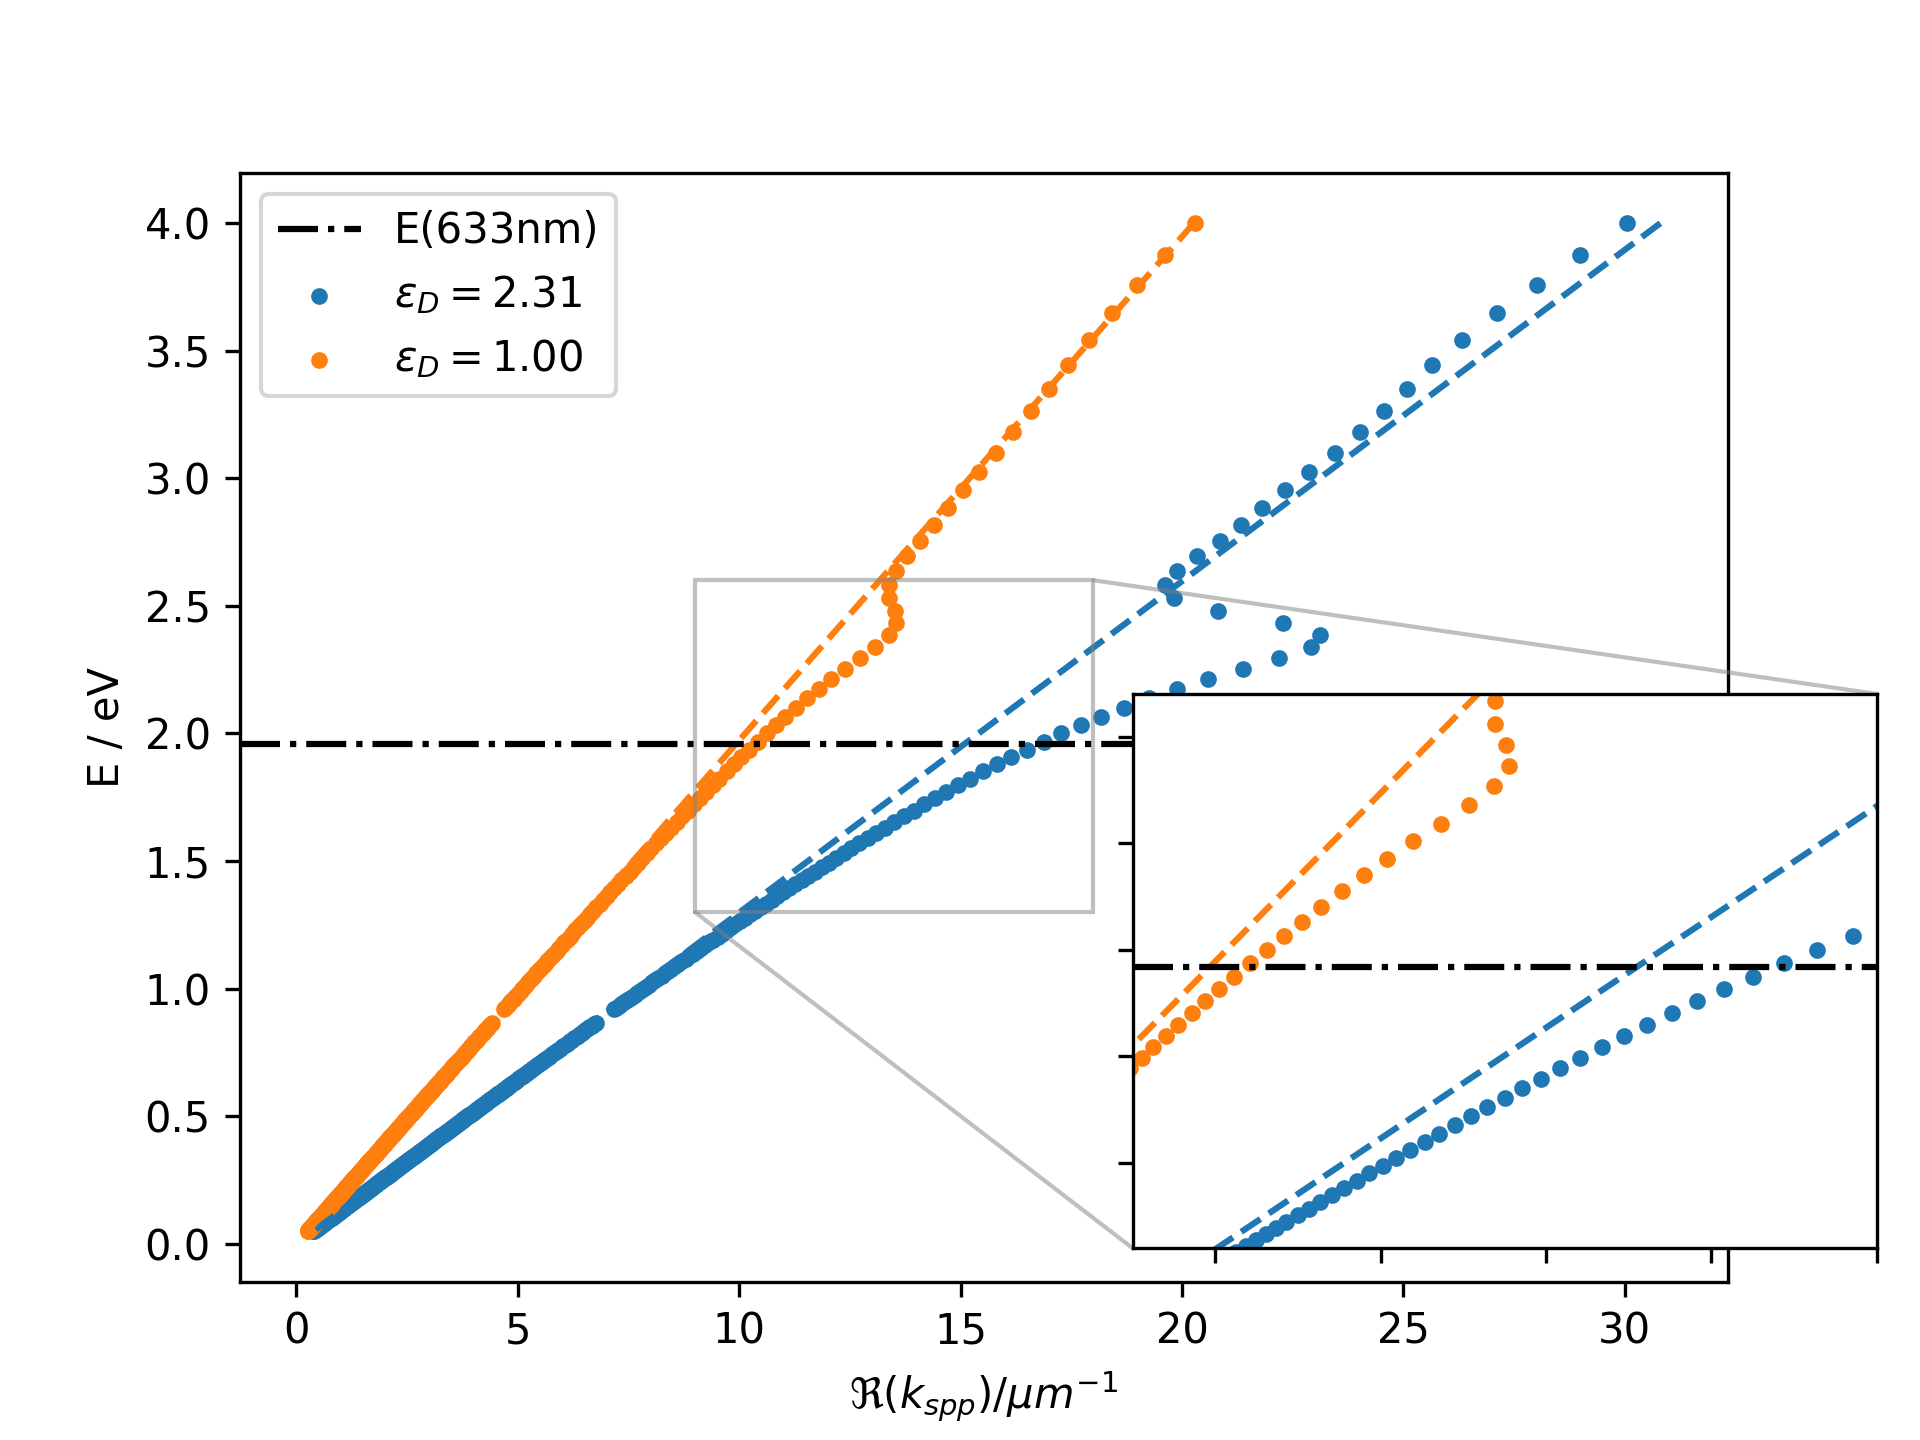
\includegraphics[width=1\textwidth]{figures/dispersion.png}
		\caption{Dispersionskurve der Gold-Vakuum und der Gold-Glas Mode. Do Lichtlinien im jeweiligen Medium sind zur Orientierung gestrichelt gekennzeichnet}		
	\end{figure}
	Diese k-Differenz sorgt dafür, dass SPPs nicht ohne weiteres von Elektromagnetischer-Strahlung des Vakuums angeregt werden können.	
		\subsubsection{Anregung}
			Um trotz der k-Differenz in der Dispersionsrelation SPPs mit elektromagnetischer Strahlung anregen zu können, ist es notwendig, den k-Wert der Anregungsstrahlung zu erhöhen. Hierfür gibt es unterschiedliche Mechanismen.
			\paragraph{Kretschman-Konfiguration}
			In der Kretschmann Konfiguration wird ausgenutzt, dass man den auf eine Ebene projizierten Anteil eines Wellenvektors durch Einfallswinkel verkleinern kann. Da der Wellenvektor allerdings vergrößert werden muss, um ein SPP mit Strahlung aus Dielektrikum anzuregen, ist es notwendig ein System mit mehr als zwei Schichten zu verwenden. Ein dünner Metallfilm wird zwischen zwei Dielektrika mit $\epsilon_{D_1} > \epsilon_{D_2}$ eingeschlossen. So ist es möglich, den Wellenvektor der Anregenden Strahlung zunächst durch Wechsel in das Dielektrikum 1 mit $\epsilon_{D_1} > \epsilon_{D_2}$ zu vergrößern, und dann durch den Einfallswinkel zu Grenzschichtebene exakt an das SPP der Mode Metall-Dielektrikum2 anzupassen. Dieses Verfahren wird bei der Kretschman-Konfiguration verwendet. Ein schematischer Aufbau der Kretschmann Konfiguration ist Abb. \ref{fig:kretschman} zu entnehmen.
				\begin{figure}[h] 
				\centering
				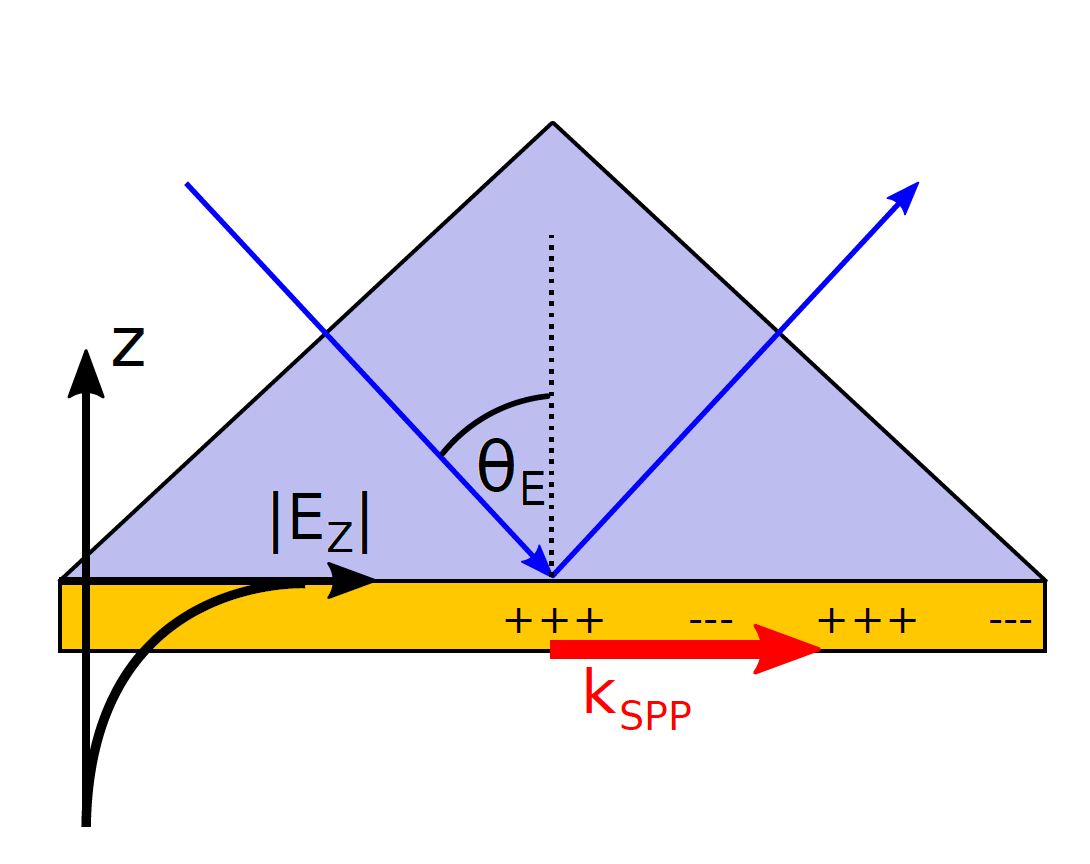
\includegraphics[width=0.5\textwidth]{figures/kretschman.png}
				\caption{Schematischer Aufbau der Kretschman-Konfiguration. Die Abbildung ist aus \cite{Jaruschewski.2020} entnommen}
				\label{fig:kretschman}
			\end{figure}
			Die Anregungsstrahlung tritt hier zunächst in das Prisma ein. Hierdurch wird der Wellenvektor der Anregungsstrahlung um $k_{D_1}=k_0\sqrt{\epsilon_{D_1}}$ vergrößert. Das Material des Prismas wird so gewählt, dass der Wellenvektor größer als der Wellenvektor des SPPs \eqref{eq:dispersion_spp} ist. Der Einfallswinkel $\theta_E$ wird so gewählt, dass die Projektion von $k_{D_1}$ auf die Goldoberfläche gerade $k_{\mathrm{spp}}$ entspricht. Es gilt also:
			\begin{align}
				\label{eq:phase_condition}
				\sin(\theta_E) &= \dfrac{\operatorname{\mathbb{R}e}\{k_{\mathrm{spp}}\}}{k_{D_1}}\\
				\Rightarrow \Aboxed{\operatorname{\mathbb{R}e}\{k_{\mathrm{spp}}\} &= \sin(\theta_E) k_0 \sqrt{\epsilon_{D_1}}}
			\end{align}
			Bei der Reflektion einer elektromagnetischen Welle an einem Metall, dringen in das Metall evaneszente Felder ein. \cite{Novotny.2012b}. Ist die Metallschicht dünn genug, haben diese evaneszenten Felder an unteren Grenzfläche des Metalls noch ausreichend Intensität, um dort ein SPP anzuregen. Dies ist möglich, da die k-Komponenten wie oben erläutert an einander angepasst worden sind. Die in Abb. \ref{fig:kretschman} gezeigte Geometrie nutzt für das Dielektrikum 1 ein Prisma, um die Einkopplung der elektromagnetischen Welle aus dem Vakuum in das Dielektrikum1 möglichst effektiv zu gestalten. Als Dielektrikum 2 wurde hier Luft verwendet.			
		
			\paragraph{Anregung an Strukturen}
			Eine weitere Möglichkeit, die Wellenvektordifferenz zu überwinden stellen scharfe Strukturen an der Metalloberfläche da. An diesen Strukturen streut das anregende Licht, und kann somit ausreichend k gewinnen, um ein SPP anzuregen. Diese Strukturen können entweder künstlich hergestellt werden, oder es werden Defekt-Stellen auf der Probe genutzt. Da die Struktur scharf im Ortsraum ist, besitzt Sie ein breites Raumfrequenzspektrum.
			... 
		\subsubsection{Leckstrahlung}
		\label{sec:leakage_radiation}
			Leckstrahlung ist der inverse Effekt zur Anregung in der Kretschmann-Konfiguration. In einem Dreischichtsystem Dielektrikum1-Metall-Dielektrikum2 kann ein an der Grenzfläche Dielektrikum1-Metall propagierendes SPP, durch evaneszente Felder, durch den Metallfilm in das Dielektrikum2 abstrahlen. Dies ist nur möglich, wenn {$\epsilon_{D_2}$ > $\epsilon_{D_1}$} ist, da sonst die Phasenanpassungsbedingung \eqref{eq:phase_condition} nicht erfüllt werden kann. Diese Strahlung tritt dann unter einem Winkel $\theta_L$ aus der Probe, so dass die Phasenanpassungsbedingung gerade erfüllt ist. Diese in das Dielektrikum 2 abgestrahlte Strahlung bezeichnet man als Leckstrahlung. Für das auftreten von  Leckstrahlung muss der Metallfilm ausreichen dünn sein, damit die evaneszenten Felder des  SPP an der zweiten Grenzschicht noch ausreichend Intensität aufweisen. Durch die Phasenanpassungsbedingung \eqref{eq:phase_condition} kann einem Bestimmten Abstrahlwinkel $\theta_L$ ein konkreter $\operatorname{\mathbb{R}e}\{k_{\mathrm{spp}}\}$ zugeordnet werden und umgekehrt. Dieser Umstand wird bei der Leckstrahlmikroskopie ausgenutzt, um den Wellenvektor des SPP zu bestimmen.
	\subsection{Plasmonischer-Spin-Hall-Effekt}
	Der Plasmonische-Spin-Hall-Effekt beschreibt, wie an einer räumlich symmetrischen Struktur angeregte SPPs, abhängig von der Polarisation der anregenden Strahlung, in unterschiedliche Richtungen propagieren. Speziell propagiert das SPP bei links-zirkular polarisierter Strahlung in eine um 180° verschiedene Richtung zu dem SPP, dass mit rechts zirkular polarisiertem Licht angeregt worden ist. 
	\subsubsection{Raumfrequenzspektrum von Elektromagnetischen-Feldern}
		Um den Plasmonischen-Spin-Hall-Effekt zu verstehen, ist es zunächst notwendig, die Raumfrequenzdarstellung von Elektromagnetischen Feldern zu verstehen. Die folgenden Ausführungen orientieren sich an \cite{Novotny.2012b}, wobei in dieser Arbeit nur der etwas einfacherer 2D-Fall ausgeführt wird.\\		
		Das Elektrische Feld am Ort $\vec{r} = \begin{pmatrix} x \\ y \end{pmatrix} $ sei durch $\vec{E}({\vec{r}})$ gegeben.
		Die Zeitabhängigkeit von $\vec{E}$ sei durch $\vec{E}({\vec{r}, t})=\operatorname{\mathbb{R}e}\{\vec{E}({\vec{r}})\exp(-i\omega t)\}$ gegeben. Dann lässt sich $\vec{E}({\vec{r}})$ durch eine Fouriertransformation in $x$-Richtung wie folgt darstellen:
		\begin{equation}
			\label{eq:Exz_fourier}
			\vec{E}(x,z) = \int_{-\infty}^{\infty}\mathrm{d}{k_x}\hat{\vec{E}}(k_x,z)\exp(ik_xx)				
		\end{equation}
		\begin{equation}
			\label{eq:EKxz_fourier}
			\hat{\vec{E}}(k_x,z) = \dfrac{1}{2\pi}\int_{-\infty}^{\infty}\mathrm{d}x\vec{E}(x,z)\exp(-ik_xx)
		\end{equation}
		Wenn wir davon ausgehen, dass das Medium entlang der $x$-Achse homogen, isotrop, linear und quellfrei ist, muss das Elektrische Feld, die sich unter diesen Bedingungen aus den Maxwellgleichungen \eqref{eq:maxwell} ergebende Helmholtz-Gleichung $(\vec{\nabla}^2+k^2)\vec{E}({\vec{r}}) = 0$, erfüllen. Einsetzen von \eqref{eq:Exz_fourier} in die Helmholtz-Gleichung ergibt mit der Definition $k_z := \sqrt{k^2-k_x^2}$ folgenden Zusammenhang:
		\begin{equation}
			\label{eq:spatial_spektrum}
		\hat{\vec{E}}(k_x,z) =\hat{\vec{E}}(k_x,z= 0) \exp(\pm ik_ z)
		\end{equation}
	Das Vorzeichen legt hier die Propagationsrichtung fest.
	Einsetzen in \eqref{eq:Exz_fourier} ergibt:
		\begin{equation}
			\label{eq:Espatial_spektrum}
			\vec{E}(x,z) = \int_{-\infty}^{\infty}\mathrm{d}{k_x}\hat{\vec{E}}(k_x,z= 0)\exp(i(k_xx\pm k_ z))
		\end{equation}
	Wenn also das Raumfrequenzspektrum für einen z-Wert bekannt ist, lassen sich die Spektren für alle anderen z-Werte gemäß \eqref{eq:spatial_spektrum} berechnen. Für einen festen Wert von $k_x$ gibt es, je nach dem ob $k_x$ größer oder kleiner als $k$ ist zwei unterschiedliche Lösungen. Wenn $k_x^2 < k^2$ ist, ist $k_z := \sqrt{k^2-k_x^2}$ eine reelle Zahl. Daher handelt es sich nach \eqref{eq:spatial_spektrum} um eine ebene Welle, die entlang der z-Achse propagiert.
	Wenn hingegen $k_x^2 > k^2$ ist, ist $k_z := \sqrt{k^2-k_x^2}$ eine imaginäre Zahl. Dann handelt es sich bei \eqref{eq:spatial_spektrum} um eine evaneszente Welle, die entlang der z-Achse exponentiell abklingt. In dem Raumfrequenzspektrum kann man also zwischen Bereichen mit Ebenen-Wellen und  Bereichen mit Evaneszenten-Wellen unterscheiden. Dieses Konzept lässt sich ohne weiteres auch auf 3 Raumdimensionen und das Magnetische Feld erweitern.
	\subsubsection{Raumfrequenzspektrum der Elektromagnetische Strahlung eines oszillierenden Dipols}
		Wenn man das oben beschriebene Verfahren auf einen Elliptisch-Polarisierten Dipol anwendet, lässt sich das Raumfrequenzspektrum bestimmen. Hier werde ich mich wieder auf den 2-Dimensionalen Fall beschränken. Das Dipolmoment sei: $$\vec{P}= \begin{pmatrix} p_x \\ p_y \end{pmatrix}$$
		$p_x$ und $p_y$ sind im allgemeinen komplexe Zahlen. So kann $\vec{P}$ auch Elliptische Polarisationen darstellen. Das Die y-Komponente des Magnetfeldes dieses Dipols lässt sich nun, wie in \cite{Novotny.2012b} und \cite{RodriguezFortuno.2013} gezeigt wird, analog zu den obigen Ausführungen in Raumfrequenzanteile zerlegen.
		\begin{equation}
			H_y(x, z) = \int_{-\infty}^{\infty}\mathrm{d}k_x\hat{H_y}(k_x, z)\exp(ik _xx)
		\end{equation}
		mit
		\begin{equation}
			\boxed{\hat{H_y}(k_x, z) = \dfrac{i\omega}{8\pi^2}\left\{p_z\dfrac{k_x}{k_z} \mp p_x\right\}\exp(ik_z|z-z_{\mathrm{Dipol}}|)}
		\end{equation}
	$z_{\mathrm{Dipol}}$ ist hierbei die Position des Dipols auf der $z-Achse$. $k_z$ lässt sich hierbei wieder über die Differenz von $k_x$ zur Gesamtwellenzahl $k$ berechnen. $k_z := \sqrt{k^2-k_x^2}$ Wenn $k_x$ schon den gesamten Anteil der Gesamtwellenzahl "aufgebraucht" wird $k_z$ imaginär und die resultierende Welle deswegen evaneszent. Wenn $k_x$ einen Anteil der Gesamtwellenzahl "übrig" lässt, bleibt $k_z$ reell und die Welle kann propagieren. Ähnlich wie bei der Leckstrahlung, ergibt sich ein durch die Phasenanpassungsbedingung ein Winkel zur $z$-Achse, unter dem die Welle mit bestimmten $k_x$ propagiert: $\theta = \arcsin(k_x/k)$. Da $k = \omega / c$  hängt das Raumfrequenzspektrum nur von dem äußeren Parameter $\omega$ bzw. $k$ ab. 
	\paragraph{Analyse des Dipol-Raumfrequenzspektrums}
		Die Analyse des Raumfrequenzspektrums erfolgt in dieser Arbeit rein quantitativ unter Verwendung von willkürlichen Einheiten.
		\subparagraph{Linear polarisierte Dipol in $x$-Richtung}
			Der Dipol sei:
			 $$\vec{P} = \begin{pmatrix} 1 \\ 0\end{pmatrix}$$
			Der Real und Imaginär Teil des Raumfrequenzspektrums in einer halben Wellenlänge unterhalb des Dipols lässt sich nun plotten. $k_x$ wurde hierbei in Einheiten von $k$ dargestellt. Die Raumfrequenzspektrums-Amplitude wurde in dem Bereich der Darstellung auf 1 normiert. Das Raumfrequenzspektrum des in x-Richtung orientierten Dipols hat eine gerade Parität, ist also achsensymmetrisch. 
		\begin{figure}[h] 
			\centering
			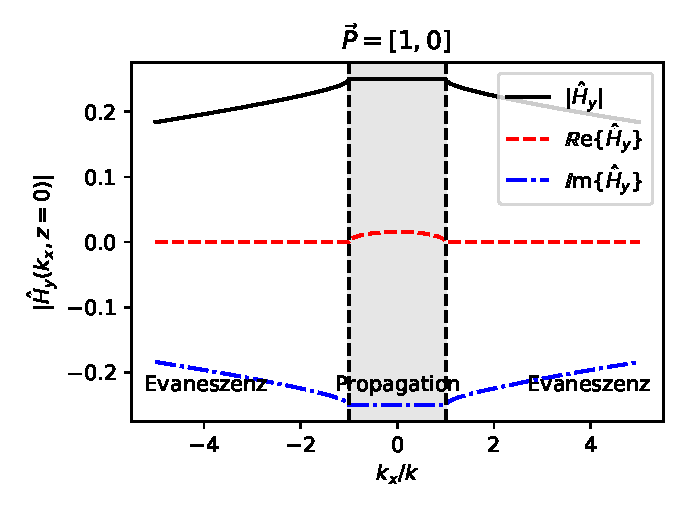
\includegraphics[width=\textwidth]{figures/spatial_spectrum_x.pdf}
			\caption{Raumfrequenspektrum in der z-Ebene, eines entlang der x-Achse orientiertem linear polarisiertem Dipol. Position des Dipols bei $z_{\mathrm{dipol}} = 0.01 \lambda$}
			\label{fig:spatial_spectrum_x}
		\end{figure}
		\subparagraph{Linear polarisierte Dipol in $z$-Richtung}
			Der Dipol sei:
			$$\vec{P} = \begin{pmatrix} 0 \\ -i\end{pmatrix}$$
			Das Raumfrequenzspektrum dieses Dipols zeigt ungerade Parität, ist also punktsymmetrisch um den Ursprung.
		\begin{figure}[h] 
			\centering
			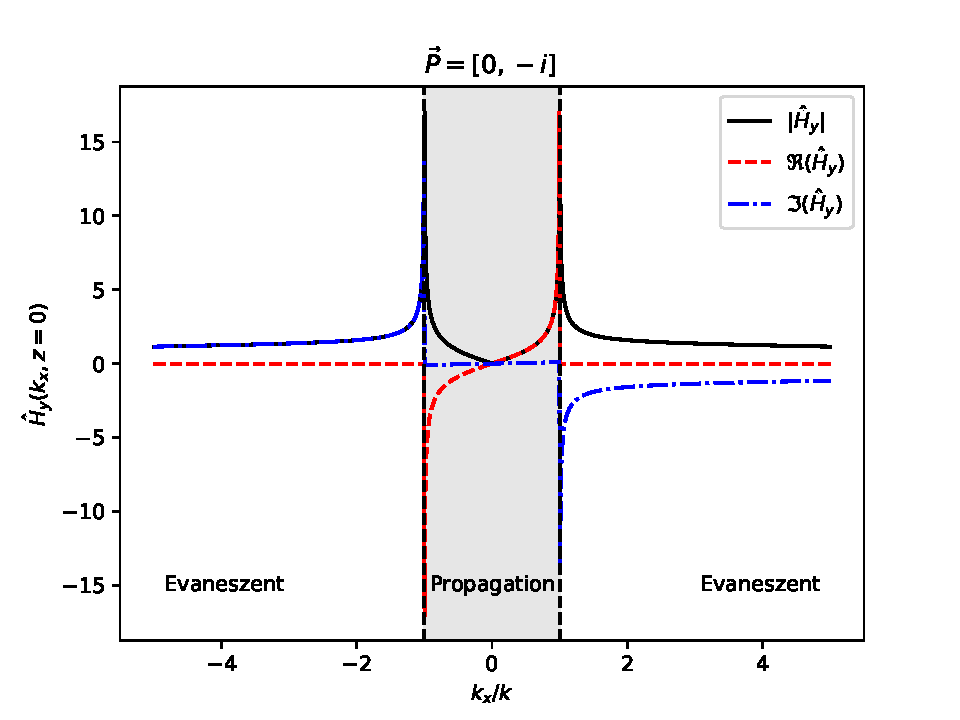
\includegraphics[width=\textwidth]{figures/spatial_spectrum_z.pdf}
			\caption{Raumfrequenspektrum in der z-Ebene, bei entlang der z-Achse orientiertem linear polarisiertem Dipol. Position des Dipols bei $z_{\mathrm{dipol}} = 0.01 \lambda$}
			\label{fig:spatial_spectrum_z}
		\end{figure}
		\subparagraph{Zirkular polarisierte Dipol}
			Der Dipol sei:
			$$\vec{P} = \begin{pmatrix} 1 \\ -i\end{pmatrix}$$
			Das Raumfrequenzspektrum aus der phasenverschobenen Überlagerung der beiden Dipole ist asymmetrisch. Im negativen x-Bereich überlagern sich die Spektren destruktiv, im positiven Bereich konstruktiv. Wenn nun sehr nah an dem Zirkular polarisierten Dipol ein Schichtsystem, dass die Anregung von SPPs unterstützt positioniert wird, kann durch den Teil des Spektrums der dem effektiven Brechungsindex der SPP-Mode entspricht ein SPP angeregt werden. Das Vorzeichen von $k_x$ entspricht hierbei der Anregungsrichtung des SPPs. Da $\hat{H}_y(k_{\mathrm{spp}}) \neq \hat{H}_y( -k_{\mathrm{spp}}) $ findet die Anregung bevorzugt in eine Richtung statt. Diese Richtung ist abhängig von dem Drehsinn des zirkular polarisierten Dipols.
			\begin{figure}[h] 
			\centering
			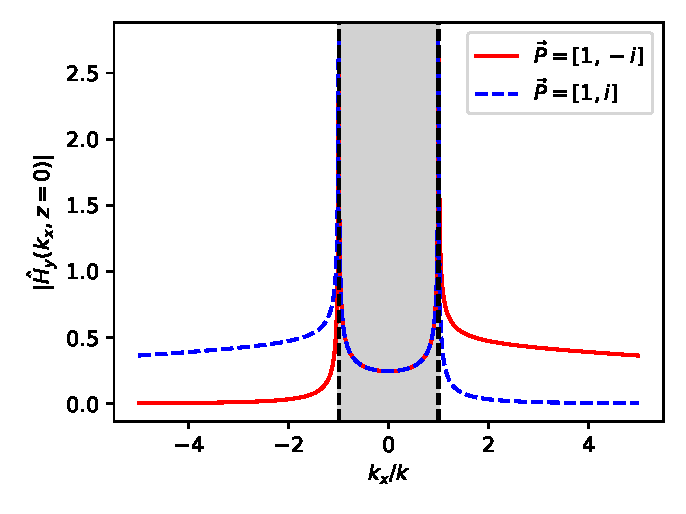
\includegraphics[width=\textwidth]{figures/spatial_spectrum_circ.pdf}
			\caption{Betrag des Raumfrequenspektrums in der z-Ebene, bei links und rechts zirkular polarisiertem Dipol. Position des Dipols bei $z_{\mathrm{dipol}} = 0.01 \lambda$}
			\label{fig:spatial_spectrum_circ}
		\end{figure}
		Das Nahfeld eine zirkular polarisiertem Dipols ist also anisotrop, obwohl das Fernfeld welches man durch substituieren von $k_x = k_o \sin(\theta)$ erhält, isotrop ist.
	
	\subsubsection{Analyse des SPP Spins}	
\section{Messung und Methoden}
\subsection{Leckstrahlmikroskopie}
	In dieser Arbeit wurde ein Leckstahlmikroskop verwendet, um den plasmonischen Spin-Hall Effekt experimentell nachzuweisen. Ein LRM hat gegenüber anderen Methoden zur Untersuchung Plasmonischer Systeme den Vorteil, dass es rein optisch arbeitet und deswegen nicht auf Vakuum-Technik angewiesen ist. Ein Leckstahlmikroskop nutzt aus, dass SPPs in einem Mehrschichtsystem wie in \Cref{sec:leakage_radiation} erläutert, Leckstrahlung unter einem spezifischen Winkel in ein Substrat abgeben können. Die Probe  wird zunächst mit einem Laser bestrahlt, und dann wird auf der Rückseite der Probe sämtliche Strahlung mit Hilfe eines Immersionsobjektives abgebildet. Aus diesem Bild wird mit Hilfe eines 4f-Aufbaus die Strahlung selektiert, die unter dem spezifischen Leckstrahlwinkel aus der Probe ausgetreten ist. So ist es möglich, die plasmonischen Anregungen ohne Störungen des direkt transmittierten Strahles zu beobachten. Das in dieser Arbeit verwendete Leckstrahlmikroskop basiert auf dem Aufbau, den Joris Jaruschewski im Rahmen seiner Masterarbeit \cite{Jaruschewski.2020} aufgebaut hat.
	\subsubsection{Immersionsobjektiv}
	Da der Winkel, unter dem die Leckstrahlung in das Dielektrikum abstrahlt größer ist, als der kritische Winkel für die Totalreflektion an der Grenzschicht Dielektrikum-Luft, muss für das Abbilden der Leckstrahlung ein Immersionsobjektiv verwendet werden. Ein Immersionsobjektiv nutzt ein Immersionsöl mit einem auf das Objektiv angepassten Brechungsindex, dass zwischen Objetiv und Probe aufgebracht wird. Durch die Adhäsions- und Kohäsionskräfte in dem Öl, ist es möglich dauerhaft einen kleinen Öltropfen zwischen Objektiv und Probe zu haben. Der Brechungsindex des Öls ist so auf das Dielektrikum der Probe angepasst, dass beide einen ähnlichen Brechungsindex aufweisen. Dadurch tritt an der Grenzfläche keine Totalreflektion auf. Durch den größen Winkel, unter dem die Leckstrahlung aus der Probe austritt ist es außerdem Notwendig, dass das Objektiv einen großen Maximalen Öffnungswinkel aufweist, damit die Leckstrahlung korrekt abgebildet wird und nicht im Inneren des Objektives an den Objektivbegrenzungen absorbiert wird. Die Fähigkeit eines Objektives Licht unter großen Winkeln zur optischen Achse aufzunehmen, lässt sich durch die Numerische Apertur $NA = n_{\mathrm{oel}}\sin\theta_{max}$ beschreiben. $\theta_{max}$ ist hierbei der halbe Maximale Öffnungswinkel des Objektives. Eine große Numerische Apertur bedeutet, dass das Objektiv Licht noch unter großen Winkel zur optischen Achse aufnehmen kann. Das in dieser Arbeit verwendete Immersionsölobjektiv war unendlich korrigiert. Das bedeutet, dass die Korrekturen der Abbildungsfehler des Objektives darauf abgestimmt worden sind, dass die Probe in der Brennweite des Objektives steht. Daher ist das Licht, welches aus dem Objektiv austritt parallel und das Zwischenbild entsteht erst im Unendlichen. Um dieses reale Zwischenbild in eine endliche Distanz zu verschieben, ist noch eine weitere Sammelinse, die sogenannte Tubuslinse notwendig. Ein unendlich korrigierte Objektiv kann auch außerhalb dieser Betriebsart verwendet werden. Allerdings treten dann zunehmend Fehler in der Abbildung auf. Der korrekte Betrieb des Objektives kann durch die Position des  1. Zwischenbildes überprüft werden.
	\subsubsection{Fourier-Optik}
	Da hinter der Probe nicht nur die Leckstrahlung, sondern auch die Strahlung des direkt transmittierten Strahls zu beobachten ist, ist es notwendig, die Leckstrahlung zu selektieren. Die Leckstrahlung tritt dank der notwendigen Phasenanpassung nur unter dem charakteristischen Winkel \eqref{eq:phase_condition} aus der Probe aus. Daher ist es möglich, die Leckstrahlung durch ihren Emissionswinkel zu identifizieren. Hierfür ist die Fourier-Optik nützlich. Eine Sammelinse besitzt die Eigenschaft, in hinteren Brennebene (BackFocalPlane BFP) ein Winkel aufgelöstes Bild von der Strahlung die sie erreicht zu erzeugen. Die Position eines Lichtstrahles in der BFP ist nur von dem Winkel des Strahls zur optischen Achse, nicht aber von der absoluten Position des Strahles abhängig. So ist es möglich bestimmte Emissionswinkel aus dem Bild herauszufiltern. 
	\paragraph{4f-Aufbau}
		Im Allgemeinen wird für diese optische Filterung ein sogenannter 4f Aufbau verwendet. Ein 4f-Aufbau besteht aus zwei Linsen mit der Brennweite $f$, die im Abstand $2f$ zueinander positioniert werden. Im Abstand $f$ von der ersten Linse wird das Zwischenbild des Immersionsobjektives positioniert. Zwischen den beiden Linsen entsteht nun das Winkelaufgelößte Fourierbild und hinter der letzten Linse entsteht wieder das Ortsbild. Wenn man nun einen Filter, der bestimmte Teile des Winkelaufgelößten Bildes herausfiltert in den Strahlgangstellt, kann im Abstand $f$ hinter der letzten Linse das Ortsbild beobachtet werden, welches nur noch aus Strahlen entstanden ist, die nicht der Filterung zum Opfer gefallen sind. Die Winkelauflösung kann auch als eine Auflösung des $k_{parallel}$ Anteils aufgefasst werden, da ein bestimmter Winkel bei gleicher Wellenlänge automatisch zu einer spezifischen k Projektion führt.
\subsection{Polarimeter}
	\subsubsection{Jones-Formalismus}
\subsection{Optischer Aufbau}
	\begin{figure}[htbp] 
	\centering
	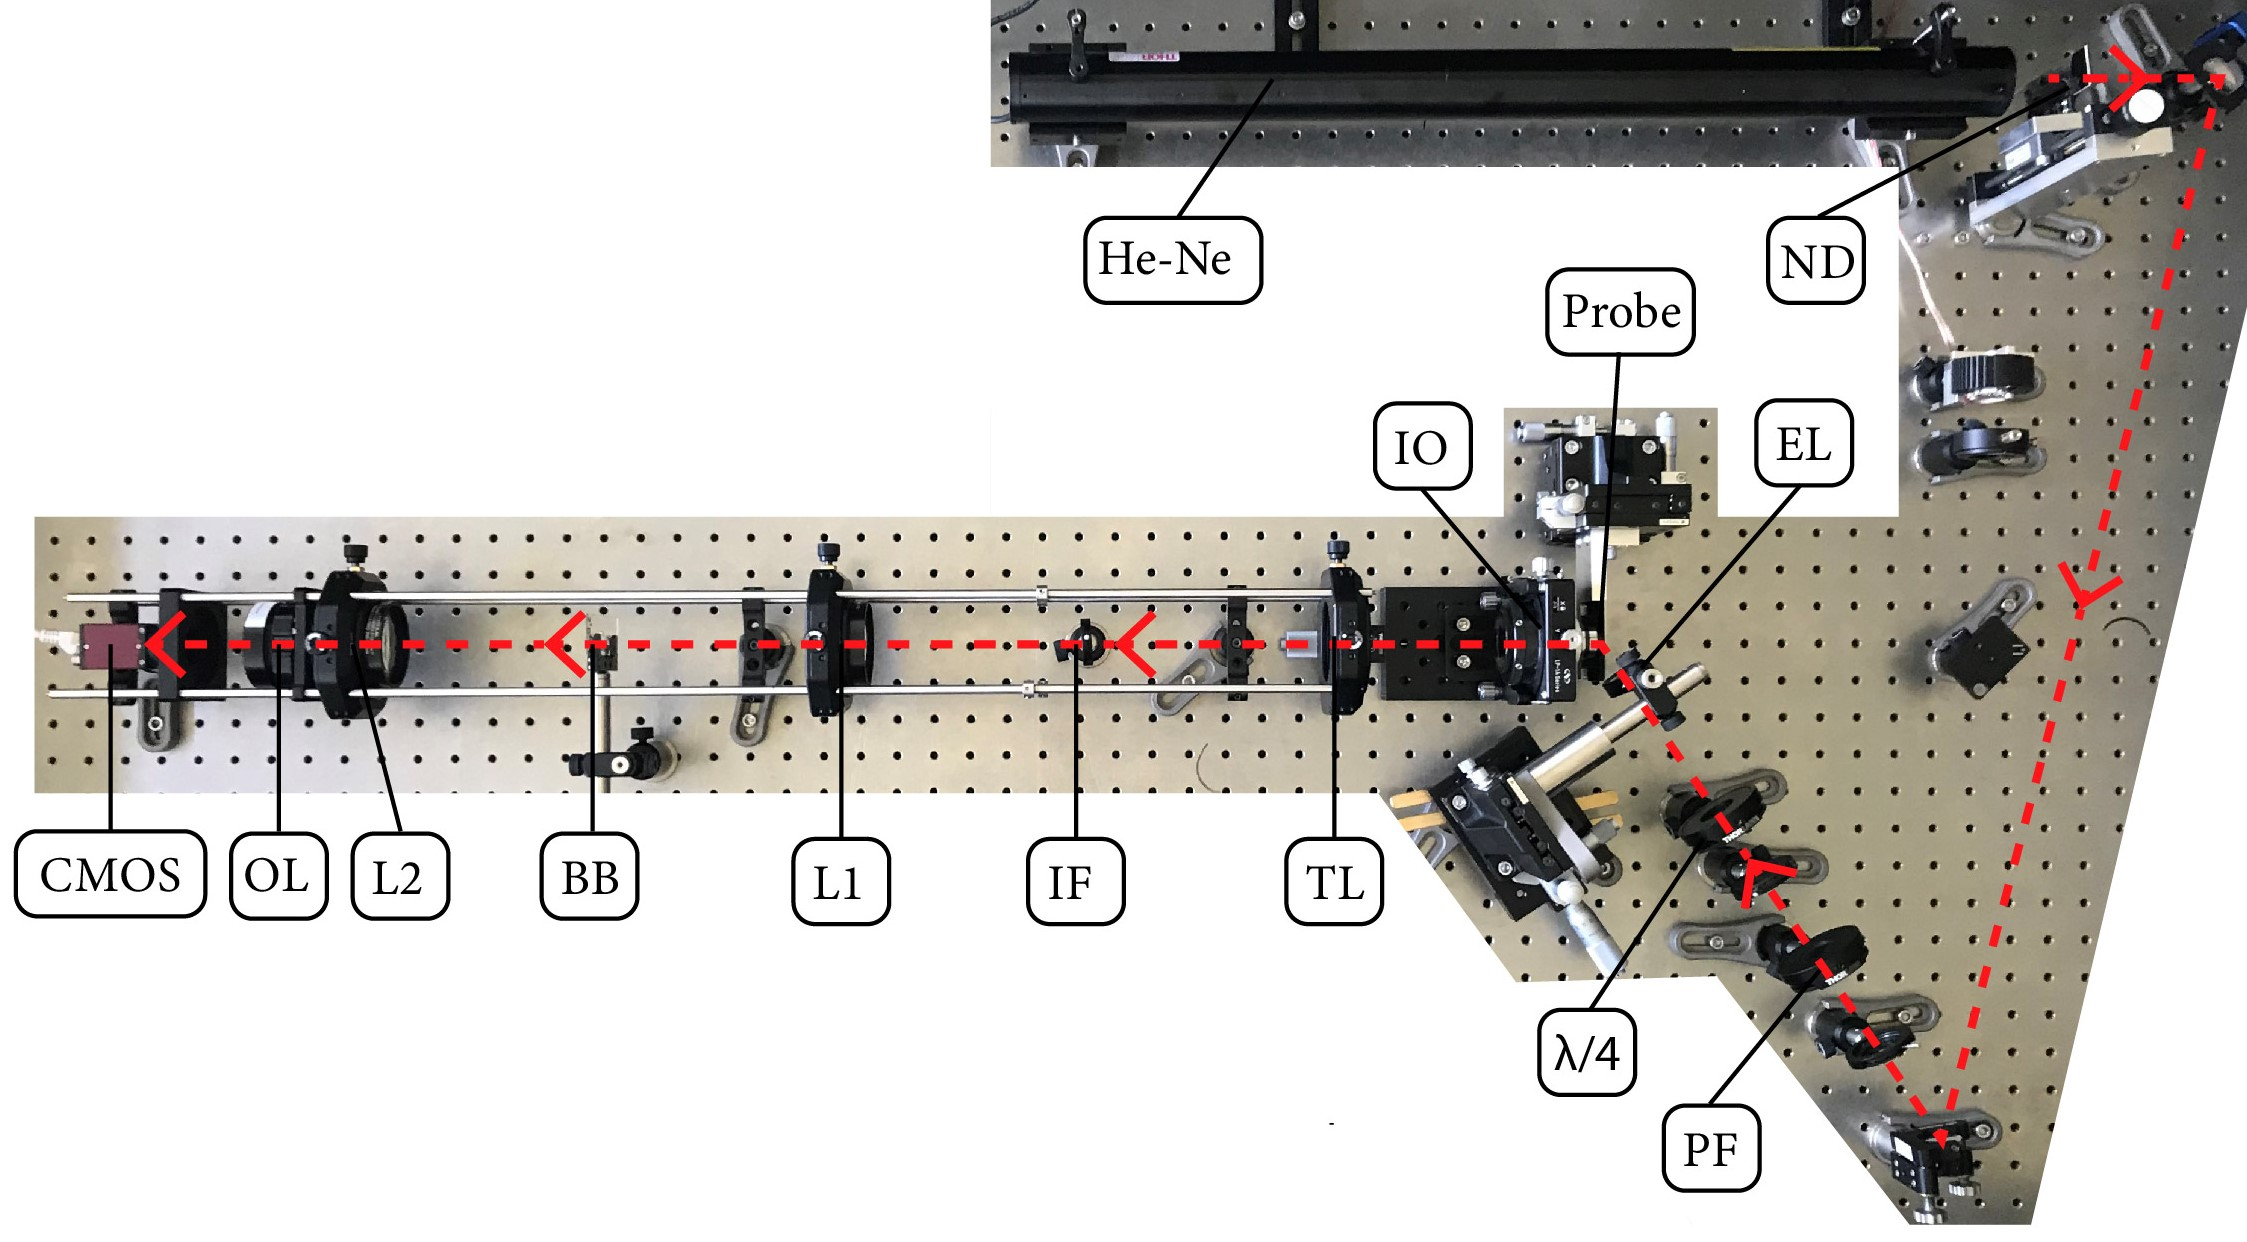
\includegraphics[width=\textwidth]{figures/aufsicht_aufbau_anotated.jpg}
	\caption{Die Komponenten des Aufbaus sind: CMOS-Sensor (CMOS), Optionale Linse (OL), Linse2 (L2), BeamBlock (BB), Linse1 (L1), ImageFilter (IF), Linse2 (L2), Imersionsobjektiv (IO), Probe, Einkoppel-Linse (EL), Verzögerungsplättchen ($\lambda/4$), Polarisationsfilter (PF), Neutraldichtefilter (ND), He-Ne Laser (He-Ne). Außerdem ist auch noch eine LED Hintergrundbeleuchtung verbaut. In Rot ist schematisch der Strahlengang des Lasers eingezeichnet}
	\label{fig:aufsicht_aufbau_anotated}
\end{figure}
\subsection{Probe}
\subsection{Justage und Kalibrierung}
\section{Ergebnisse und Diskussion}
	\subsection{Bestimmung des Polarisationszustandes}
		\subsubsection{Modellierung Jones-Polarimeter}
		\subsubsection{least-square-fit}
	\subsection{Bestimmung des Kontrastverhältnisses linkes/rechtes SPP}
		\begin{figure}[htbp] 
		\centering
		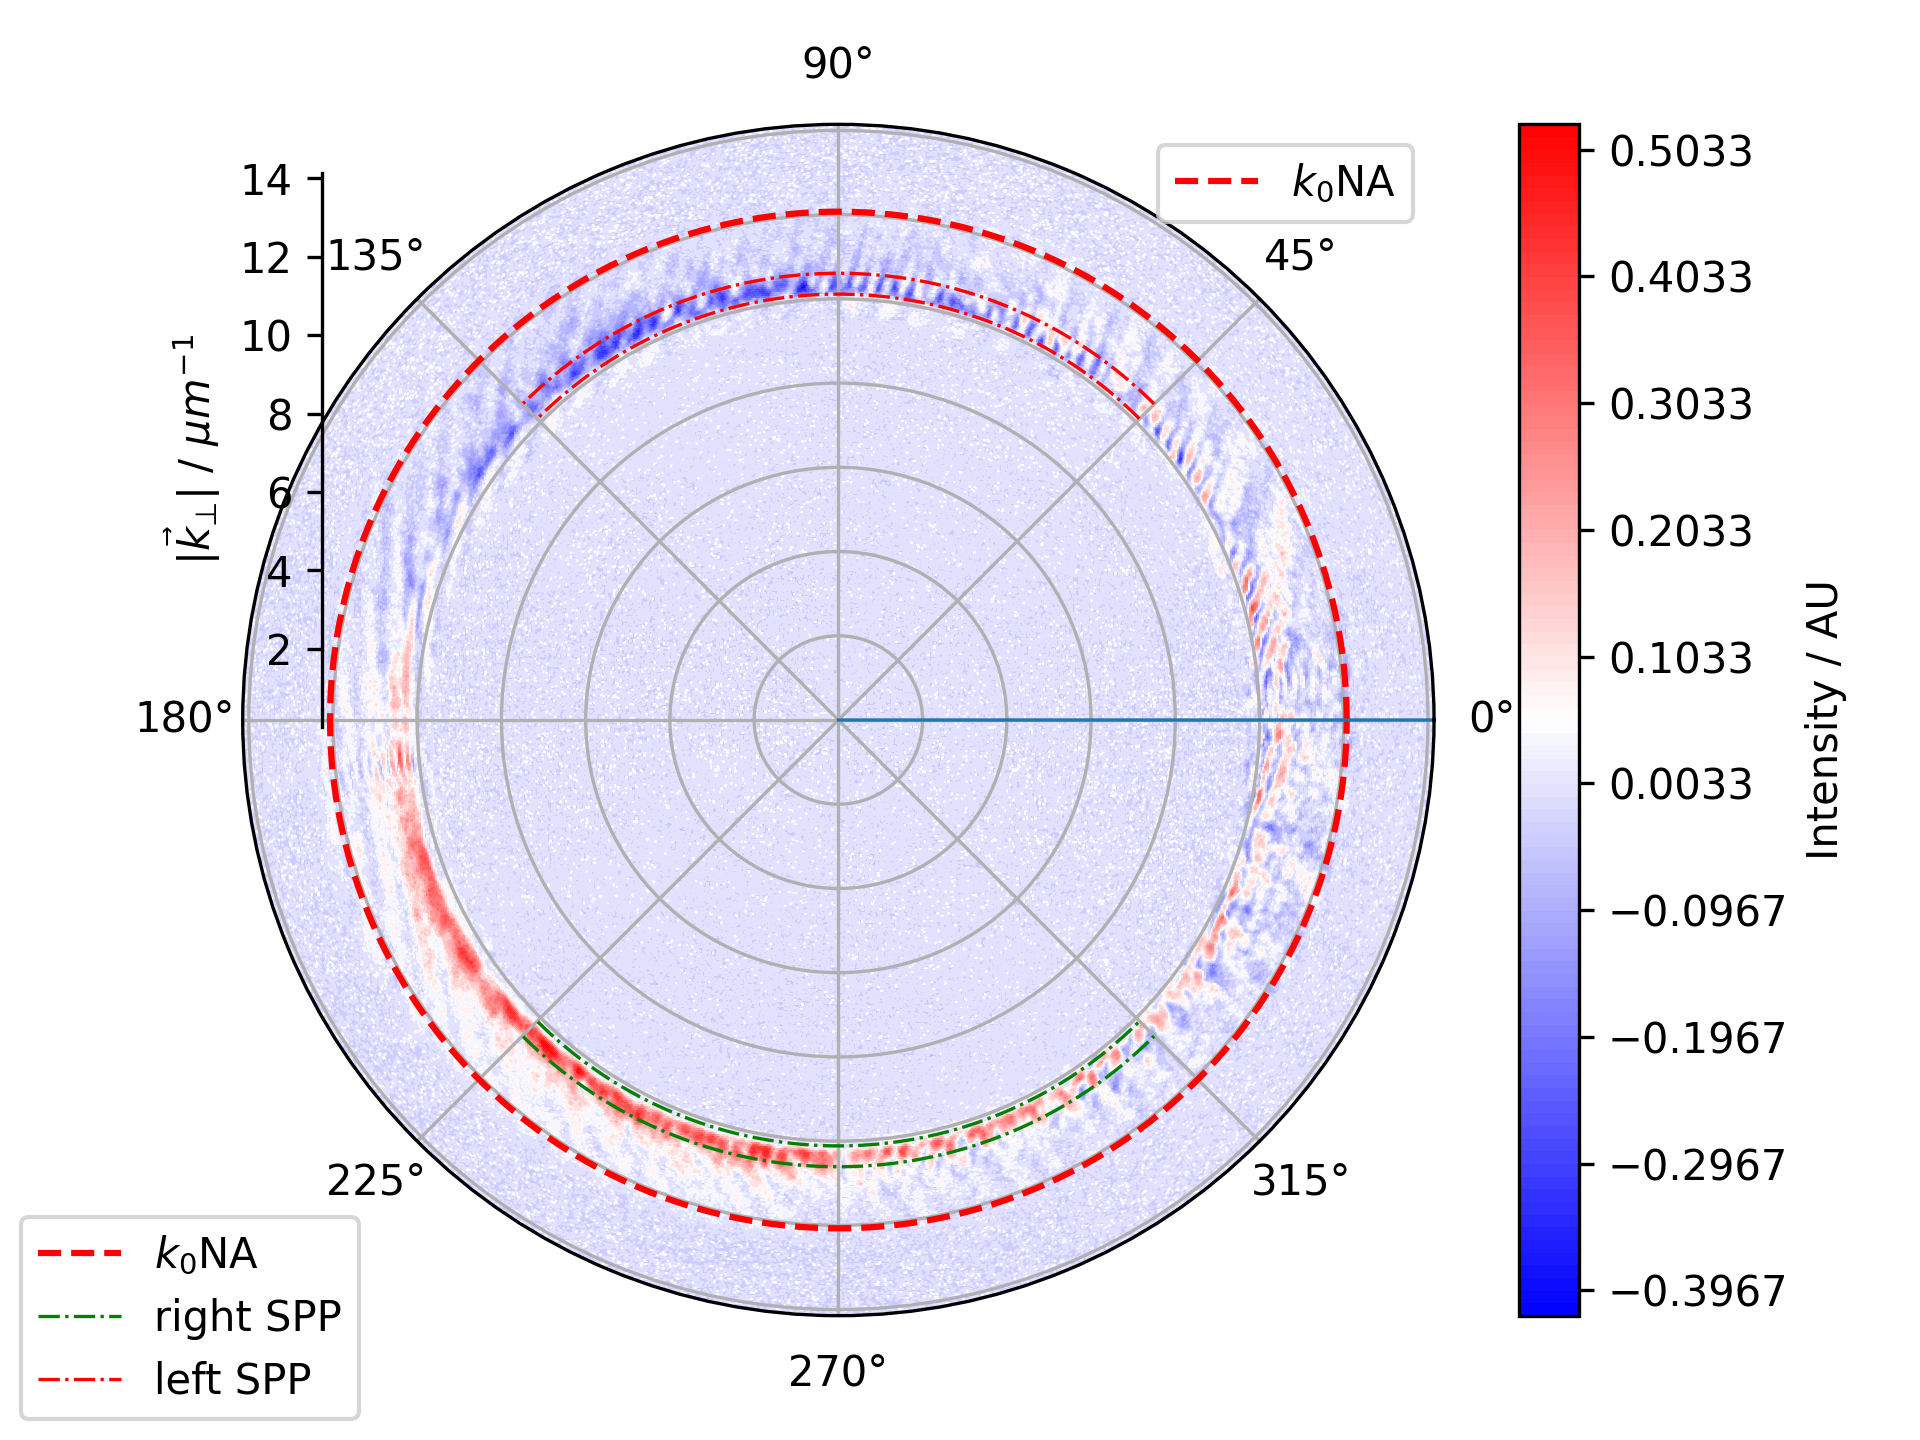
\includegraphics[width=\textwidth]{figures/polar_diff_mask4.png}
		\caption{Die Abbildung zeigt in rot und grün die Integrationsmasken. Außerdem zeigt sie die Differenz zwischen dem Winkel 44 und 134}
		\label{fig:polar_diff_mask4}
		\end{figure}
	\begin{figure}[htbp] 
	\centering
	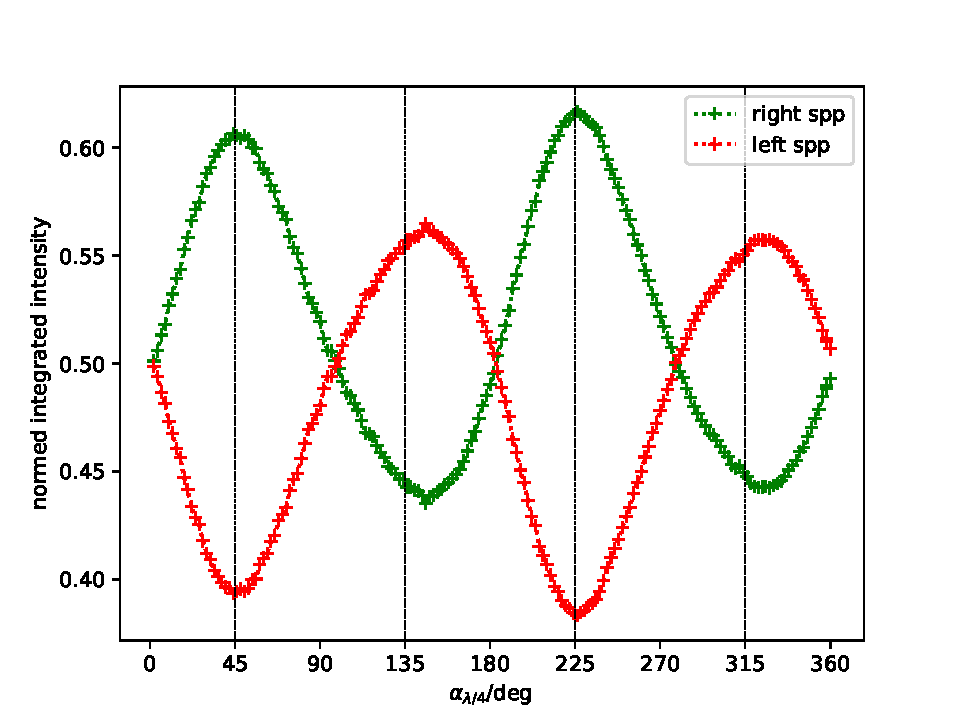
\includegraphics[width=\textwidth]{figures/integrated_intesity4.pdf}
	\caption{Kontrastverhältnis}
	\label{fig:integrated_intesity4}
\end{figure}
	\subsection{Diskussion}
\section{Zusammenfassung und Ausblick}
\newpage
\bibliography{bib}
	
\end{document}